% ****** Start of file apssamp.tex ******
%
%   This file is part of the APS files in the REVTeX 4.2 distribution.
%   Version 4.2a of REVTeX, December 2014
%
%   Copyright (c) 2014 The American Physical Society.
%
%   See the REVTeX 4 README file for restrictions and more information.
%
% TeX'ing this file requires that you have AMS-LaTeX 2.0 installed
% as well as the rest of the prerequisites for REVTeX 4.2
%
% See the REVTeX 4 README file
% It also requires running BibTeX. The commands are as follows:
%
%  1)  latex apssamp.tex
%  2)  bibtex apssamp
%  3)  latex apssamp.tex
%  4)  latex apssamp.tex
%
\documentclass[%
 reprint,
%superscriptaddress,
%groupedaddress,
%unsortedaddress,
%runinaddress,
%frontmatterverbose, 
%preprint,
%preprintnumbers,
%nofootinbib,
%nobibnotes,
%bibnotes,
 amsmath,amssymb,
 aps,
%pra,
%prb,
%rmp,
%prstab,
%prstper,
%floatfix,
]{revtex4-2}

\usepackage{graphicx}% Include figure files
\usepackage{dcolumn}% Align table columns on decimal point
\usepackage{bm}% bold math
%\usepackage{hyperref}% add hypertext capabilities
%\usepackage[mathlines]{lineno}% Enable numbering of text and display math
%\linenumbers\relax % Commence numbering lines

%\usepackage[showframe,%Uncomment any one of the following lines to test 
%%scale=0.7, marginratio={1:1, 2:3}, ignoreall,% default settings
%%text={7in,10in},centering,
%%margin=1.5in,
%%total={6.5in,8.75in}, top=1.2in, left=0.9in, includefoot,
%%height=10in,a5paper,hmargin={3cm,0.8in},
%]{geometry}

\begin{document}

\preprint{APS/123-QED}

\title{Analysis of the near-side Ridge in high-multiplicity pp collisions \\ at $\sqrt{s}=13TeV$ via Momentum-Kick model}% Force line breaks with \\
\thanks{A footnote to the article title}%

\author{Ann Author}
 \altaffiliation[Also at ]{Physics Department, XYZ University.}%Lines break automatically or can be forced with \\
\author{Second Author}%
 \email{Second.Author@institution.edu}
\affiliation{%
 Authors' institution and/or address\\
 This line break forced with \textbackslash\textbackslash
}%

\collaboration{MUSO Collaboration}%\noaffiliation

\author{Charlie Author}
 \homepage{http://www.Second.institution.edu/~Charlie.Author}
\affiliation{
 Second institution and/or address\\
 This line break forced% with \\
}%
\affiliation{
 Third institution, the second for Charlie Author
}%
\author{Delta Author}
\affiliation{%
 Authors' institution and/or address\\
 This line break forced with \textbackslash\textbackslash
}%

\collaboration{CLEO Collaboration}%\noaffiliation

\date{\today}% It is always \today, today,
             %  but any date may be explicitly specified

\begin{abstract}
An article usually includes an abstract, a concise summary of the work
covered at length in the main body of the article. 
\begin{description}
\item[Usage]
Secondary publications and information retrieval purposes.
\item[Structure]
You may use the \texttt{description} environment to structure your abstract;
use the optional argument of the \verb+\item+ command to give the category of each item. 
\end{description}
\end{abstract}

%\keywords{Suggested keywords}%Use showkeys class option if keyword
                              %display desired
\maketitle

%\tableofcontents

\section{\label{sec:level1} Introduction}

Ridge structure refers to the shape of ‘ridge’ that appears at long-range.
Previously, Ridge structure was observed in the case of heavy-ion collisions such as PbPb \cite{ref1, ref2, ref3, ref4, ref5, ref6, ref7, ref8, ref9, ref10, ref11} 
and AuAu collisions \cite{ref12, ref13, ref14, ref15, ref16, ref17, ref18, ref19, ref20, ref21, ref22, ref23, ref24, ref25, ref26, ref27}. 
In this case, they can be understood by collective motion, based on hydrodynamics theory, because it is enough to create high-temperature and high-density environment.
And this is the hint of Quark-Gluon Plasma (QGP) state.
Recently, however, in the case of high multiplicity of the proton-proton collision, ridge structure is also observed.
It was expected that small system could not create such the environment. 
In this case, the medium doesn’t create such the collective motion.
Therefore, we will analyze the ridge structure in high multiplicity proton-proton collision at 13TeV, using the Momentum-Kick model \cite{Wong_2, Wong_3, Wong_4, Wong_5}.

The Momentum-Kick model is based on pure kinematics between Jet and Medium particles.
The Momentum-Kick model assumes that near-side Jet partons transfer their momentum to medium.
That model uses the process to explain ridge structure at near-side, which is $\Delta \phi \sim 0$.
In this paper, we will analyze the ridge structure using the Momentum-Kick model in high multiplicity proton-proton collision 
at 13TeV from ALICE, CMS, and ATLAS experiments.


\section{Momentum-Kick Model}


The Momentum-Kick model explains the results of experiments at near-side region, through the behavior of near-side jet fragments kicking the medium parton. 
This model is successfully applying the experimental results in AuAu at 200GeV \cite{Wong_1} and PbPb at 2.76TeV \cite{PbPb}, etc. 
We expect that kinematics behavior is more dominant in the small system than heavy-ion collision.
Hence, the Momentum-Kick model will be expected to describe successfully in proton-proton collision at 13TeV in high-multiplicity.

In the Momentum-Kick model, total yield is expressed as follows:
\begin{equation} \label{equation:eq1}
\begin{split}
\left[\frac{1}{N_{\text{trig}}}\frac{dN_{\text{ch}}}{p_tdp_td\Delta\eta d\Delta\phi}\right]_{\text{total}}^{\text{AA}} ={}  \\
\left[{\frac{2}{3}}f_R\left\langle N_k\right\rangle\frac{dF}{p_tdp_td\Delta\eta d\Delta\phi}\right]_{\text{Ridge}}^{\text{AA}} 
+ \left[f_J\frac{dN_{\text{jet}}^{\text{pp}}}{p_tdp_td\Delta\eta d\Delta\phi}\right]_{\text{Jet}}^{\text{AA}},
\end{split}
\end{equation}
which is the sum of ridge and jet fragments.
$\Delta \eta $ and $\Delta \phi$ are the difference of $\eta$ and $\phi$ between jet and the other particles.
$f_J$ is the average survival coefficient of jet fragments, 
$f_R$ is the average survival factor of ridge particles, 
and $\left\langle N_k\right\rangle$ is the average of kicked partons per-trigger particle.

In the Momentum-Kick model, jet component is written as follow:
\begin{equation} \label{equation:eq2}
\frac{dN_{\text{jet}}^{\text{pp}}}{p_tdp_td\Delta\eta d\Delta\phi}
= N_{\text{jet}}\frac{e^{\left[ \left( m-\sqrt{m^2+p_t^2} \right) \middle/ T_{\text{jet}}\right]}}{T_{\text{jet}}\left(m+T_{\text{jet}}\right)}\times
\frac{1}{2\pi\sigma_\phi^2}e^{ \left. -\left[\left(\Delta\phi\right)^2+ \left(\Delta\eta\right)^2\right] \middle/ 2\sigma_\phi^2 \right. },
\end{equation}
where $N_{\text{jet}}$ is the total number of jet particles, $T_{\text{jet}}$ is the temperature of jet partons, and $\sigma_\phi$ is the jet cone width, which can be parameterized as:
\begin{equation} \label{equation:eq3}
\sigma_\phi= \left. \sigma_{\phi_0}m_a \middle/ \sqrt{m_a^2+p_T^2} \right. .
\end{equation}
In the equation \ref{equation:eq2} the exponential term is a Gaussian distribution, which indicates that jet particles are concentrated in the center of the jet cone. 
Since near-side jet rarely exists in long-range which is $\left|\Delta\eta\right|>1.6$, jet component is not included in this analysis.

The Momentum-Kick model explains ridge component via soft scattering model:
\begin{equation} \label{equation:eq4}
\frac{dF}{p_tdp_td\eta d\phi}
= \left[\frac{dF}{p_{ti}dp_{ti}dy_id\phi_i} \frac{E}{E_i} \right]_{\mathbf{p}_i=\mathbf{p}-\mathbf{q}}\times\sqrt{1-\frac{m^2}{\left(m^2+p_t^2\right){\cosh}^2y}}.
\end{equation}
$ dF / p_{ti}dp_{ti}dy_id\phi_i $ is the normalized initial parton distribution, which implies the distribution before freezing out.
$\mathbf{p}_i$ is the initial parton momentum, which is the shifted momentum as $\mathbf{p}_i=\mathbf{p}-\mathbf{q}$.
$\mathbf{q}$ denotes an average value of kicked momentum.
The transverse momentum of initial particles is written as follows:
\begin{equation} \label{equation:eq5}
p_{ti}^2=p_{tf}^2-\frac{2p_{tf} q \cos\left(\Delta\phi\right)}{\cosh{\left(\eta_{\text{jet}}\right)}}+\frac{q^2}{\cosh^2{\eta_{\text{jet}}}}.
\end{equation}
Since most of near-side jet is concentrated in the $\Delta\eta,\Delta\phi \sim 0$ region, we set $\eta_{\text{jet}}=0$.
$E/E_i$ insures conservation of energy between initial and final partons.
$\sqrt{ \left. 1- m^2 \middle/ \left(m^2+p_t^2\right){\cosh}^2y \right.}$ converts the rapidity into pseudo-rapidity.

The initial parton momentum distribution is expressed as follow:
\begin{equation} \label{equation:eq6}
\frac{dF}{p_{ti}dp_{ti}dy_id\phi_i}=A_{\text{ridge}}\left(1-x\right)^a\frac{e^{ \left. -\sqrt{m^2+p_{ti}^2} \middle/ T \right. }}{\sqrt{m_d^2+p_{ti}^2}}.
\end{equation}
In equation \ref{equation:eq6}, $A_{ridge}$ is the normalization constant satisfying:
\begin{equation} \label{equation:eq7}
\int{A_{ridge}\left(1-x\right)^a\frac{e^{ \left. -\sqrt{m^2+p_{ti}^2} \middle/ T \right. }}{\sqrt{m_d^2+p_{ti}^2}}}p_{ti}dp_{ti}dy_id\phi_i=1.
\end{equation}
$T$ is the one of major parameters to explain momentum distribution, indicating the temperature of medium particles.
Since pions are expected to take up the majority of partons, we set $m$ as the pions mass.
$m_d$ is a cut-off parameter that prevents divergence at small $p_{Ti}$.
$a$ is a fall-off parameter, which determines the rate of decrease of $1-x$ distribution.
$m_d$ and $a$ are set the same as references \cite{PbPb, Wong_1} for the general application of the Momentum-Kick model \cite{Wong_1}.
Also, $x$ is the light-cone variable written as follow:
\begin{equation} \label{equation:eq8}
x=\frac{\sqrt{m^2+p_{ti}^2}}{m}e^{\left|y_i\right|-y_b},
\end{equation}
where $y_b$ is the rapidity of the beam defined as $y_b=\cosh^{-1}{\sqrt{s_{NN}}/2m_N}$. $m_N$ is the mass of beam particles, set as the proton mass.


\section{LHC Detector}
We verify our model in ALICE, CMS and ATLAS experiments \cite{alice,cms,atlas}. The conditions of data analyzed in these experiments are summarized in Table \ref{table:range}.

\begin{table}[h!]
  \centering
  \begin{tabular}{||c c c c||} 
   \hline
   & ALICE & CMS & ATLAS \\ [0.5ex] 
  \hline\hline
  $\Delta \eta $ range & $1.6<|\Delta \eta |<1.8$ & $2<|\Delta \eta |<4$ & $2<|\Delta \eta |<5$ \\ 
  Multiplicity & $0\sim0.1\%$ & $N>105$ & $N>90$ \\
  $p_T$ range & $1<p_T<4$ & $0.1<p_T<4$ & $0.5<p_T<5$ \\[1ex]
  \hline
 \end{tabular}
 \caption{The ranges of data in ALICE, CMS, and ATLAS experiments \cite{alice, cms, atlas}}
 \label{table:range}
\end{table}

Moreover, references \cite{alice, cms, atlas} used different methods in analyzing their data.
In ALICE and CMS analysis, they used Zero Yield At Minimum (ZYAM) method, a traditional experimental analysis method.
In this method, the minimum value is set to zero by subtracting.
However, ATLAS used the peripheral subtraction method.
It takes the ridge component from the experiment data by subtracting the peripheral component,
which is low multiplicity pp collisions, to check the flow effect.
However, we apply ZYAM method when we use ATLAS experiment data for consistency.


\section{Fitting results}
We compare physical parameters in ridge component of Momentum-Kick model at STAR AuAu at 200GeV \cite{Wong_1}, CMS PbPb at 2.76TeV \cite{PbPb}
and pp at 13TeV, in which ALICE, CMS and ATLAS data are used from reference \cite{alice, cms, atlas}.

\begin{table}[h!]
  \centering
  \begin{tabular}{||c c c c||} 
   \hline
    & AuAu 200GeV & PbPb 2.76TeV & pp 13TeV \\ [0.5ex] 
   \hline\hline
   T (GeV) & 0.5 & 0.6 & 0.65 \\
   q (GeV) & 1.0 & 0.7 & 0.9 \\ 
  $f_R \left\langle N_k \right\rangle$ & 4 & $20.2e^{-\frac{1.395}{\left\langle p_{T}^{trig} \right\rangle}-0.207{\left\langle p_{T}^{trig} \right\rangle}}$ & $0.83+0.5{p_T}^2$ \\[1ex]
   \hline
 \end{tabular}
 \caption{Physical parameters in ridge component of momentum kick model.}
 \label{table:param}
\end{table}

Since $T$ is higher as center of mass energy gets bigger, $T$ becomes higher from 0.5 GeV at AuAu to 0.6 GeV at PbPb. 
For the same reason, $T$ is 0.65 GeV at pp collision at 13TeV, which is 8.3\% higher than PbPb at 2.76TeV.

The medium density from PbPb is expected to be denser than that from AuAu.
Since the number of kicks between medium partons is higher, the average of momentum transfer per kick in PbPb is lower than in AuAu,
as can be seen, $1.0 \rightarrow 0.7$ GeV in Table \ref{table:param}.
However, the medium from pp at 13TeV is expected less dense than that from PbPb, even though the center of mass energy is higher,
$q$ becomes higher from 0.7 GeV at PbPb collision to 0.9 GeV at pp collision. 

% Since particles that received more momentum will escape faster, $f_R$ is exponentially increased by $p_T$, reference \cite{PbPb} used $e^{-A/p_T}$ (A is a constant) form.
% We also the similar exponential form $e^{Ap_T}$ form, because we want to maximize the effect of the survival ratio of the high $p_T$ particles.

% However, $\langle N_k \rangle$ is more dependent on the total number of particles that have reached a detector.
% In the case of heavy-ion collisions, density of the initial partons is very high.
% The number of collisions between mediums is different as $p_T$, since high momentum particles are reach to detector faster than low momentum particles.
% Therefore, $\langle N_k \rangle$ from PbPb collision at 2.76TeV is $Ae^{-B \times p_T}$ form.
% However, since pp collision at 13TeV creates lower density than heavy-ion collision, the number of collisions between medium doesn't care about the velocity of particles.
% Therefore, we use $\langle N_k \rangle$ as a constant.

% As a result, we set $f_R \langle N_k \rangle = A+B{p_T}^2$ form (A and B are constants), 
% and fig.\ref{figure:frnk} is a graph compared to references \cite{Wong_1, PbPb}.

Since the initial parton momentum distribution is normalized, $f_R \langle N_k \rangle$ describe the number of particles,
which is reached to the detector.
We assumed that particles with high energy can reach the detector more easily.
Since the square of pT means energy, we set $f_R \langle N_k \rangle = A+B{p_T}^2$ term (A and B are constants).
we also check $f_R \langle N_k \rangle = Ae^{Bp_T}$ form, which is also proportional to $p_T$.
Fig.\ref{figure:frnk} is a graph compared to references \cite{Wong_1, PbPb}.


\begin{figure}[ht]
\centering
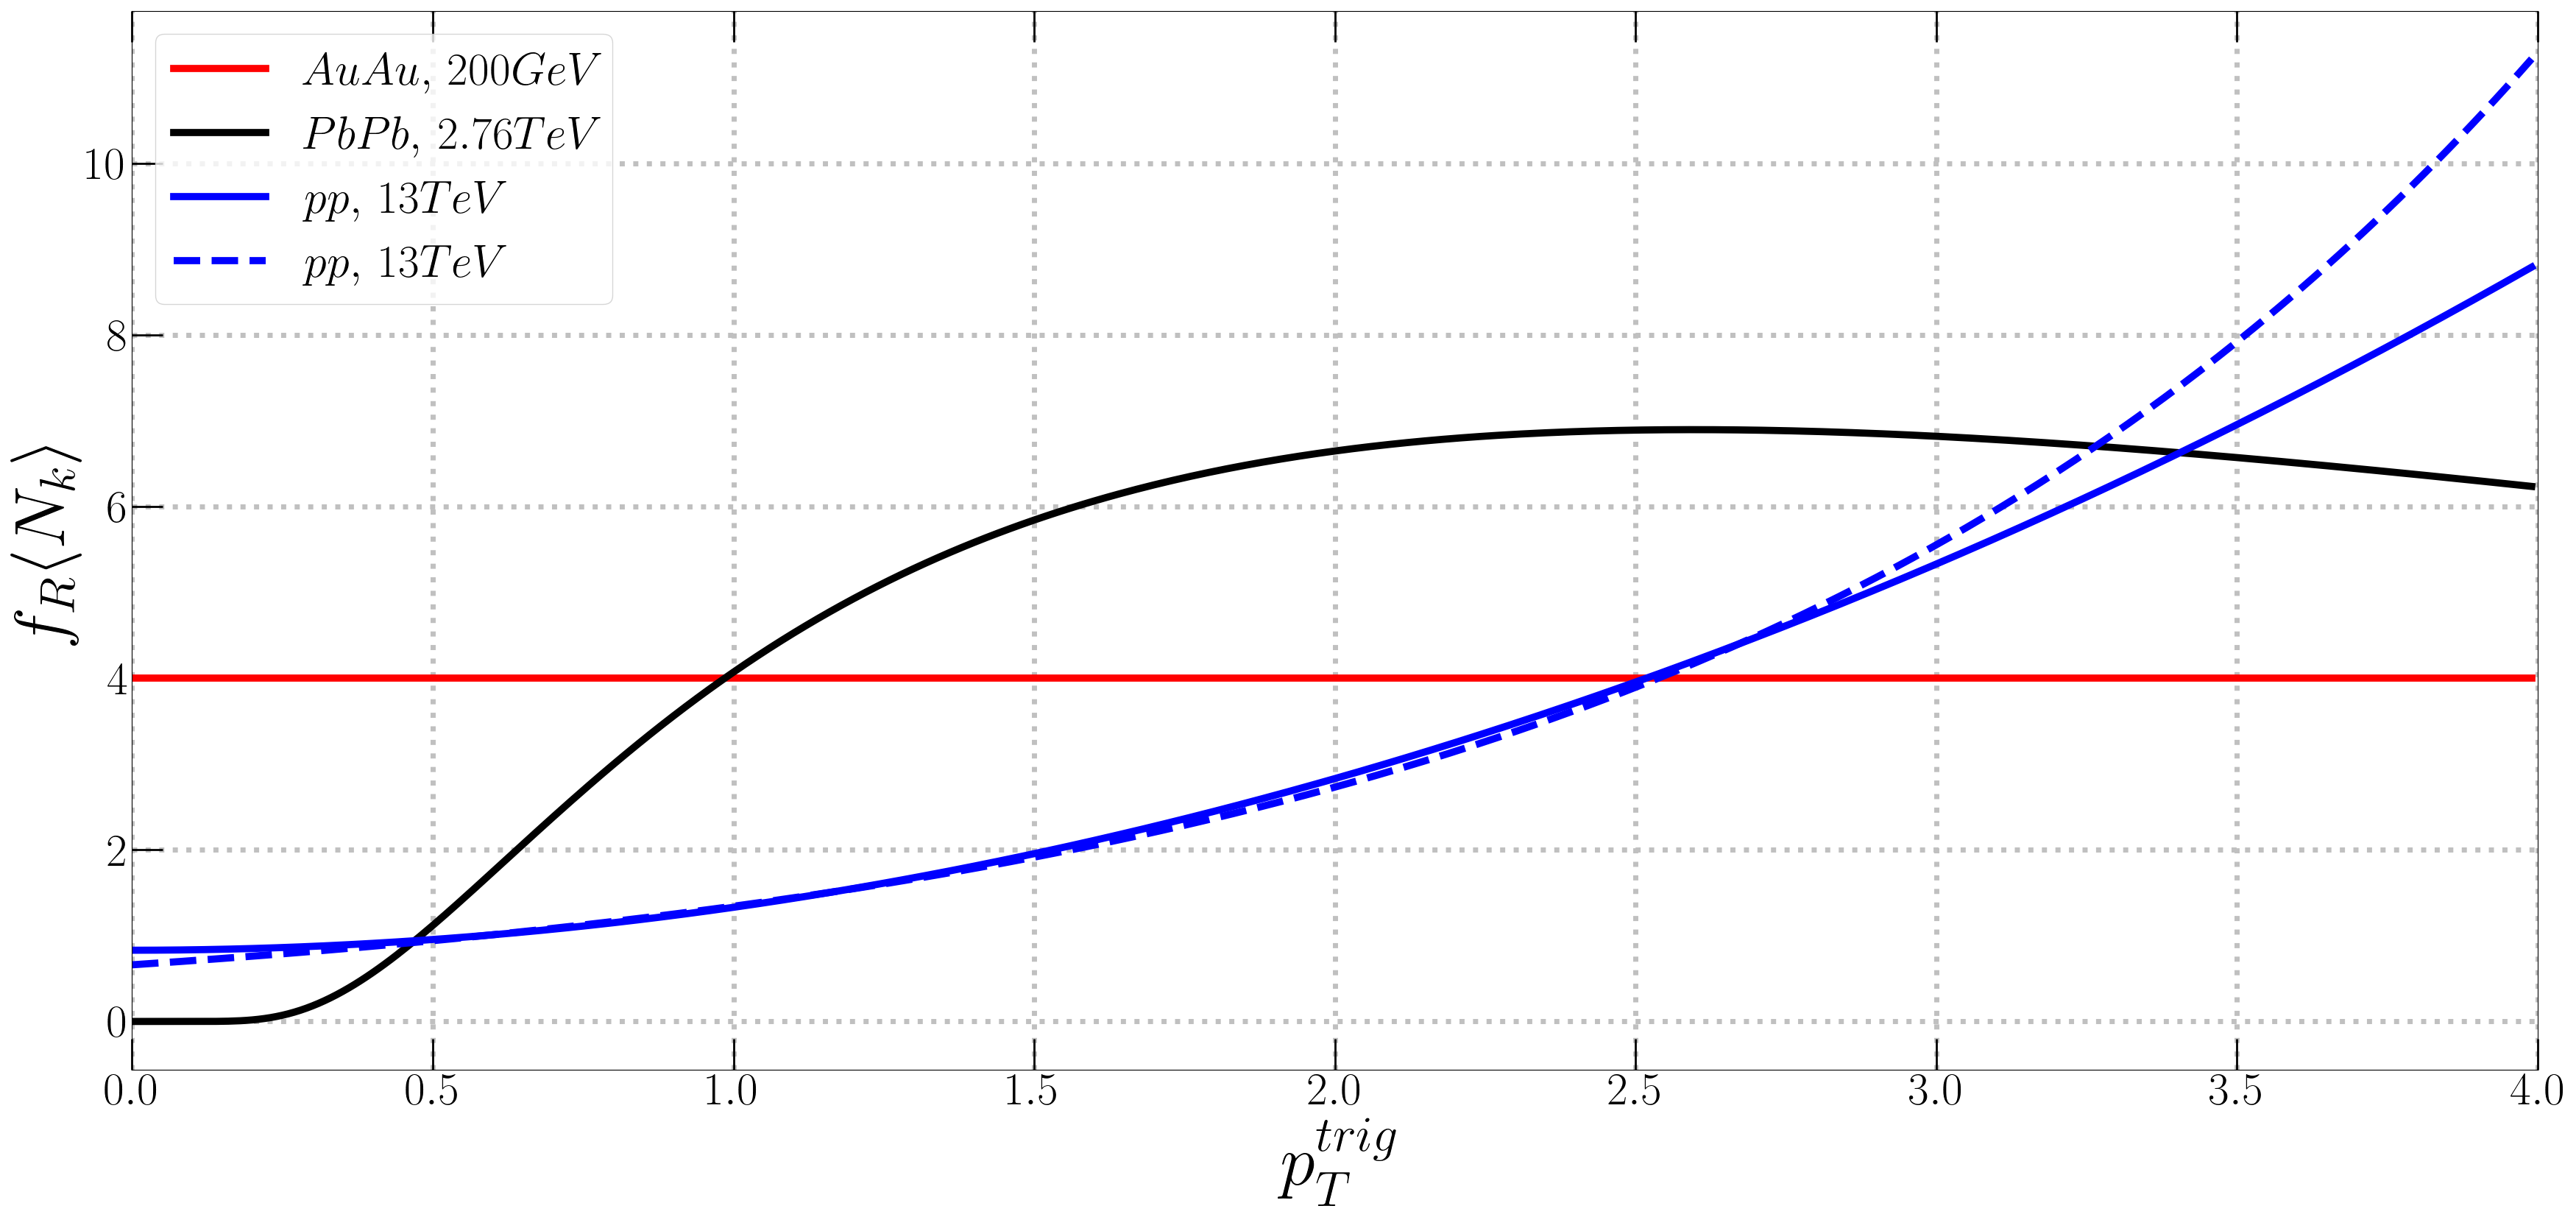
\includegraphics[width=12cm, height=6cm]{Paper_frnk}
\caption{Graphs of $f_R \left\langle N_k \right\rangle$ fitting results of AuAu 200GeV, PbPb 2.76TeV and pp 13TeV for $p_{T}^{trig}$.
Dashed line of blue color is $A+B{p_T}^2$, solid line of blue color is $Ae^{Bp_T}$ term.}
\label{figure:frnk}
\end{figure}

The range of $p_T^{\text{trig}}$ in PbPb at 2.76TeV is changing while range of $p_T^{\text{assoc}}$ kept constant.
However, in pp at 13TeV, when the range of $p_T^{\text{trig}}$ changes, the range of $p_T^{\text{assoc}}$ changes together.
Hence, it is difficult to compare directly, but it is possible to see trend.

First of all, in the case of AuAu collision at 200GeV, since it has low energy, $f_R \langle N_k \rangle$ doens't have $p_T$ dependence.
For this reason, it has the highest at the low $p_T$.
However, in PbPb collision at 2.76TeV, since density of medium is very high, Jet particles transfer their momentum to medium many times.
Therefore, many of medium partons, which are received momentum as $q$, are more likely to reach the detector.
As a result, $f_R \langle N_k \rangle$ at PbPb collision has the highest at the mid-range of $p_T$.
In the case of pp collision at 13TeV, since medium density is low, Jet particles kick medium particles a little time.
Therefore, because of maximize the effect of survival ratio at high $p_T$, $f_R \langle N_k \rangle$ is the highest in high $p_T$.
However, since $A+B{p_T}^2$ and $Ae^{Bp_T}$ have similar trend in $p_T<4$, we have to check higher $p_T$ range data.

We fit the momentum kick model to the ALICE, CMS, and ATLAS proton-proton Collision 13TeV at high-multiplicity \cite{alice, cms, atlas}. 

\begin{figure}[ht]
\centering
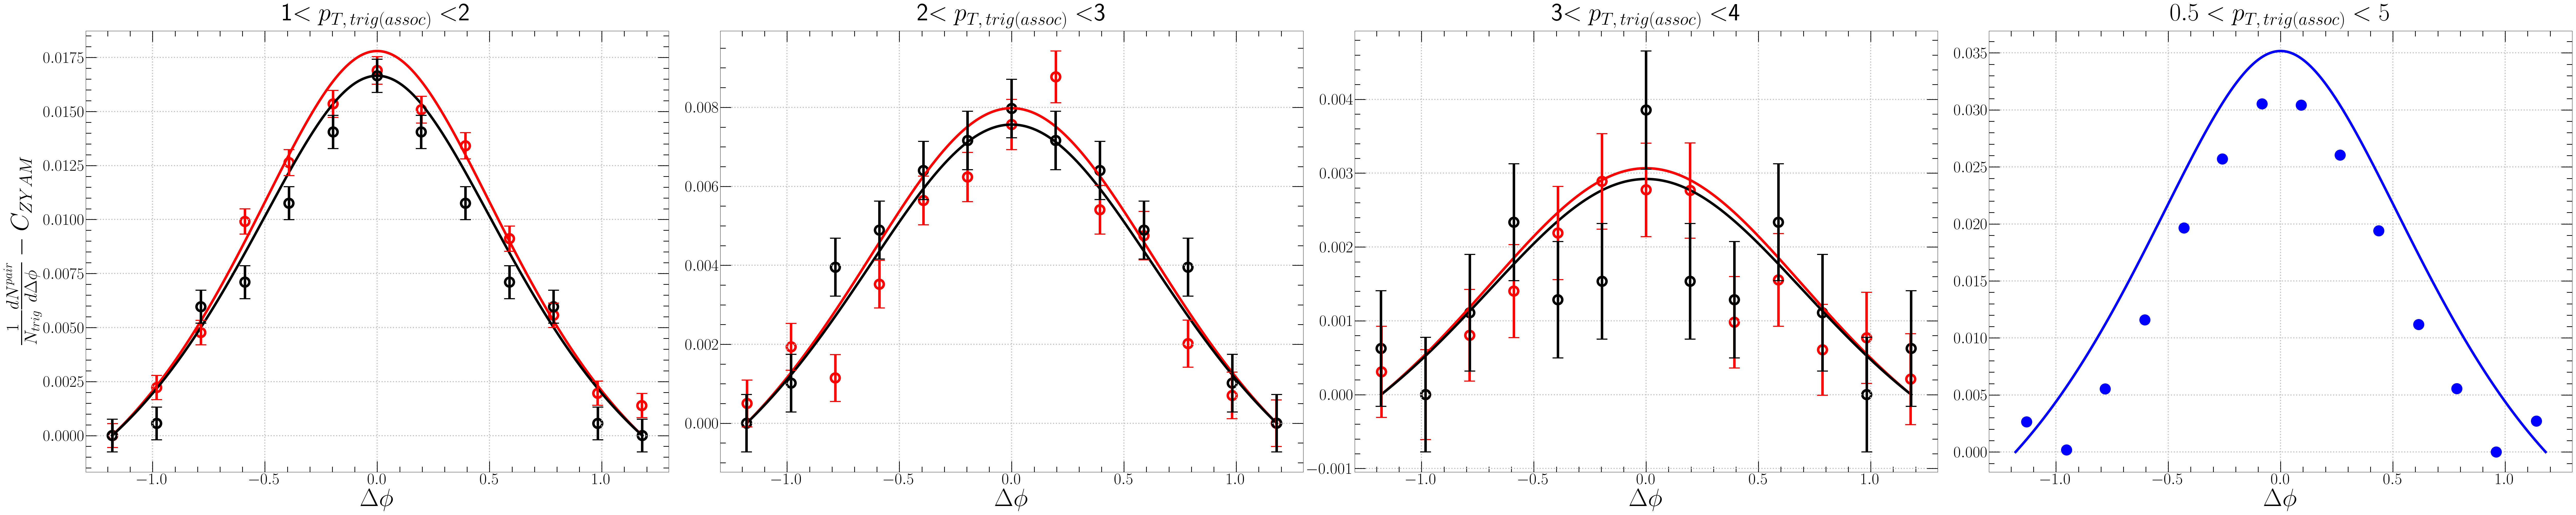
\includegraphics[width=16cm, height=3.5cm]{Paper_phiCorr}
\caption{Result for $\Delta \phi$ correlation. All curves are momentum kick model result, plots are experimental data.
Red is the result from ALICE, black is from CMS and blue is from ATLAS.
For ALICE and CMS data, we draw the case of $1<p_T<2, 2<p_T<3, 3<p_T<4$. And in ATLAS data, we draw for $0.5,p_T<5$.}
\label{figure:phicorr}
\end{figure}

\begin{figure}[ht]
\centering
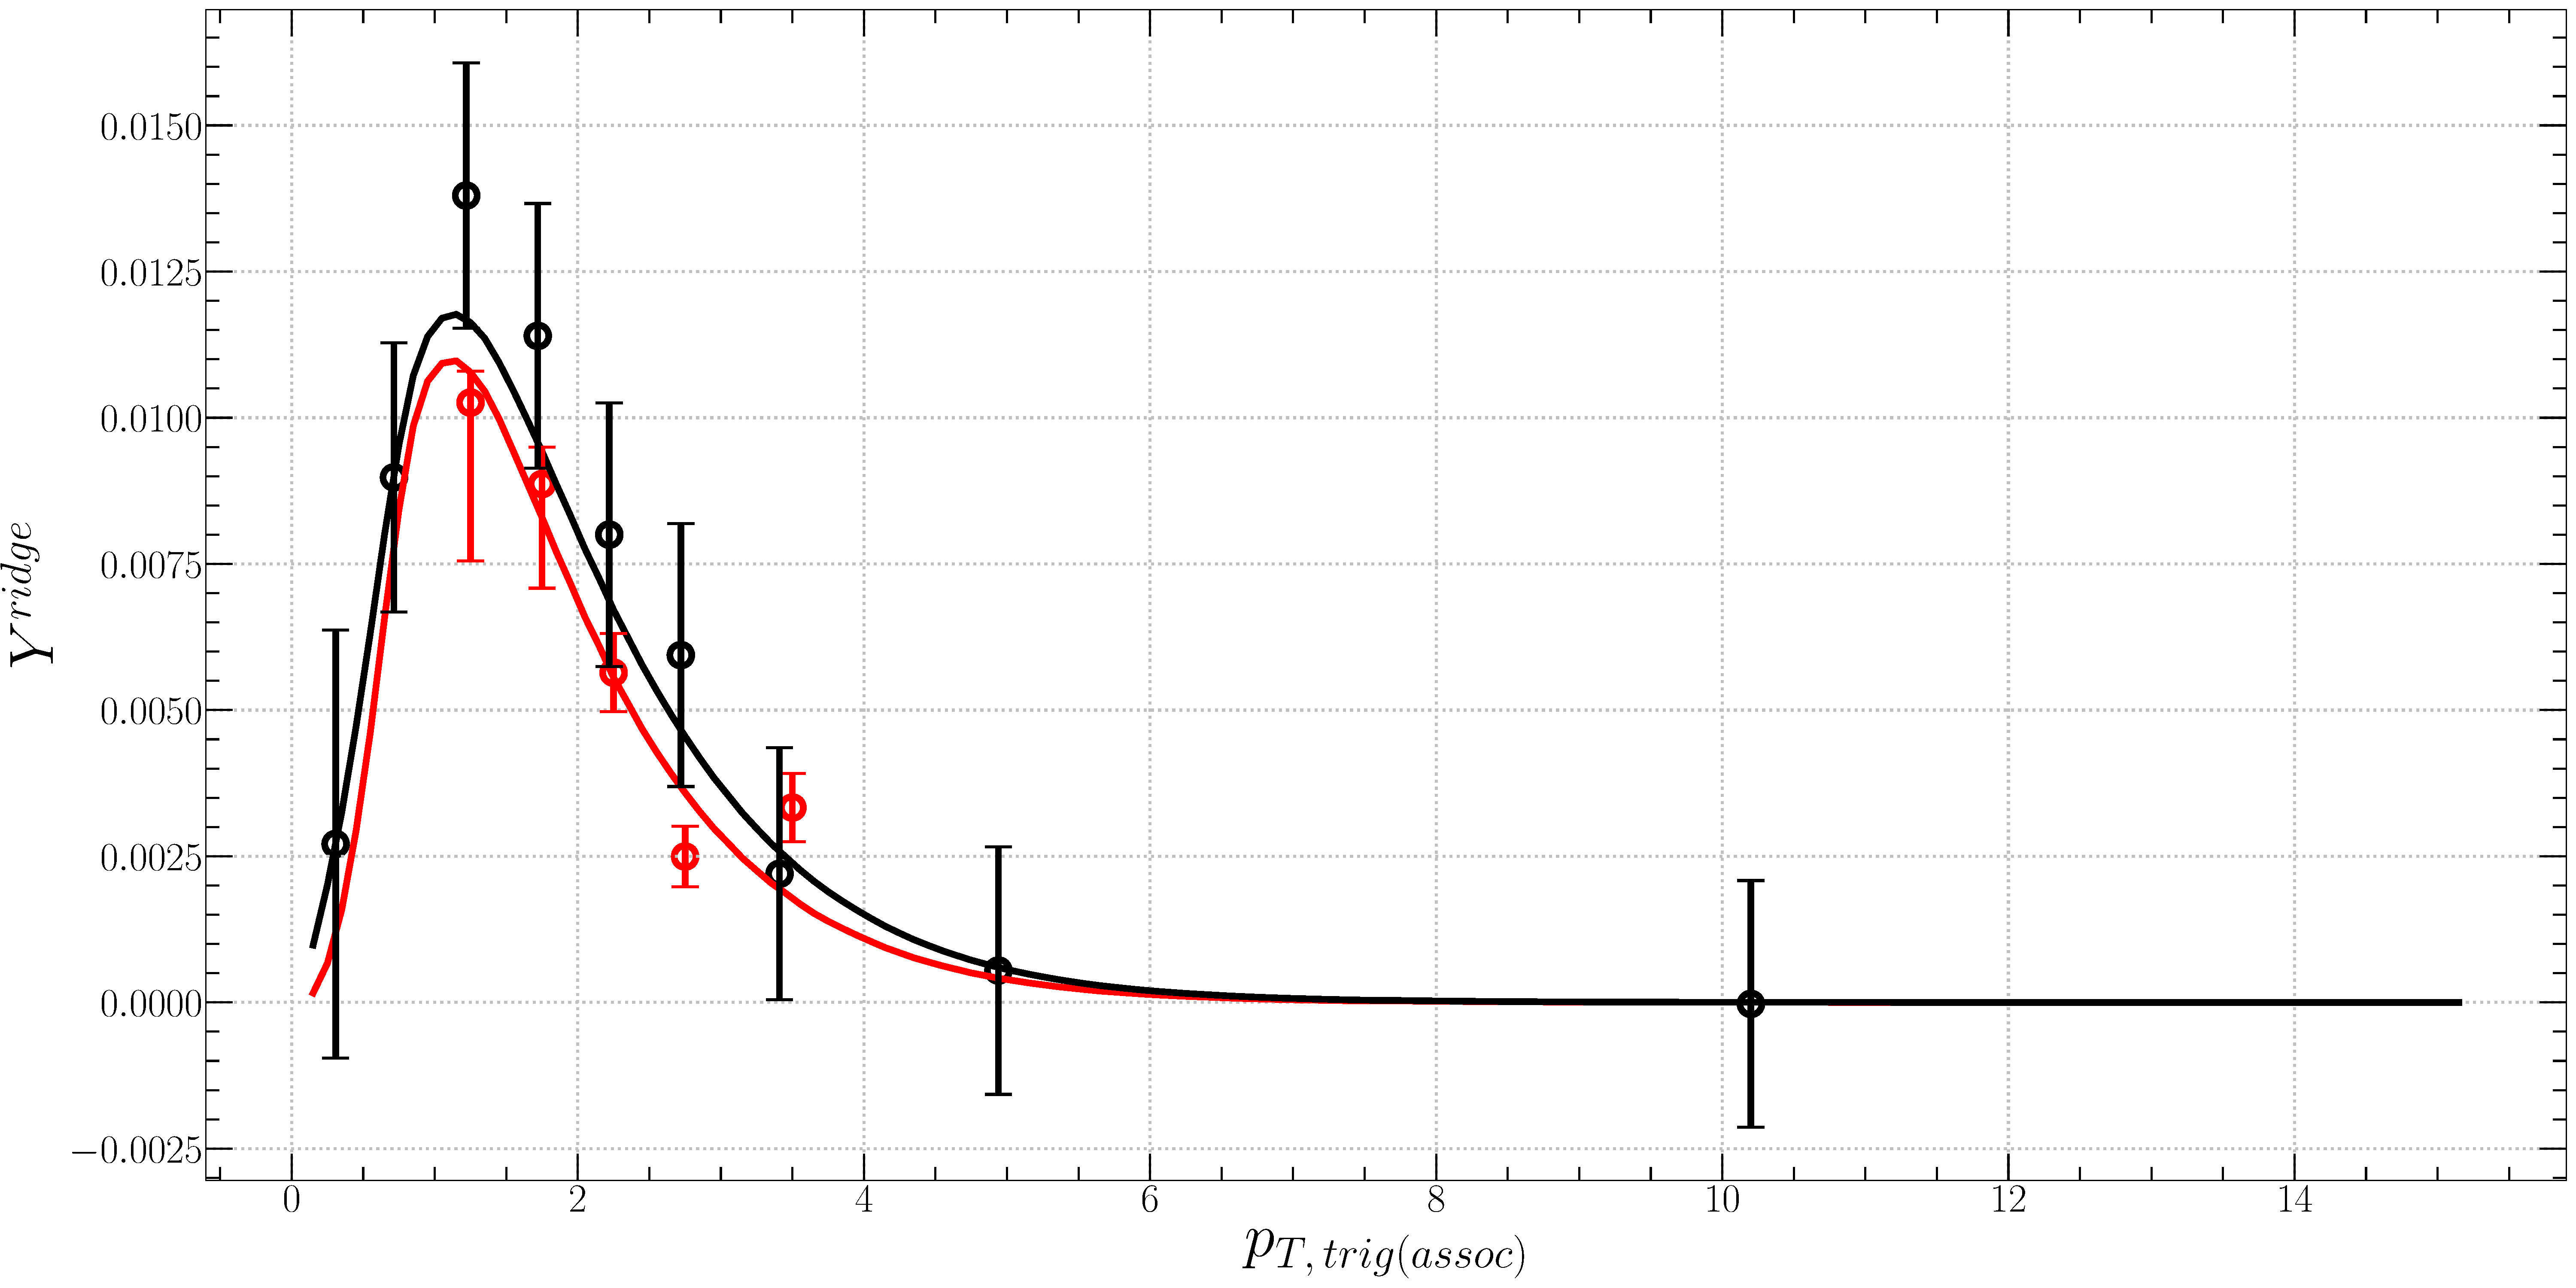
\includegraphics[width=8cm, height=4cm]{Paper_pTdis}
\caption{$p_T$ distribution for only ALICE and CMS result. ATLAS couldn’t draw because of no result for $p_T$ distribution.}
\label{figure:pTdis}
\end{figure}

In $\Delta\phi$ correlation, we draw Momentum-Kick model result and LHC data. 
The solid line is the Momentum-Kick model, and circles are the LHC data. And red color is ALICE data and Momentum-Kick model, 
black is for CMS, and blue is for ATLAS. LHC data is well described via momentum kick model all of $p_T$ range.
Since partons are kicked as $q$ by Jet particles, the theoretical ridge yield must show a peak in $q$. 
However, since $f_R \langle N_k \rangle $ is exponentially increased for $p_T$, the position of the peak is moved to an area where the $p_T$ is larger. 
In this paper, the peak is made around $p_T=1.2$. Therefore, the momentum kick model can describe well in $p_T$ distribution, too.


\section{Conclusion}

We have analyzed the long-range near-side proton-proton collision at $\sqrt{s_{NN}}=13TeV $in ALICE, CMS and ATLAS data. 
Since the small system has a less flow effect than heavy-ion collision, the Momentum-Kick model is expected to be applied well in the high multiplicity pp collision. 
We apply our model in high multiplicity pp collision at 13TeV data from all 3 collaboration, altogether. 
As a result, we obtain $T=0.65\, GeV,\, q=0.9\, GeV,\, f_R\left\langle N_k\right\rangle=0.66e^{0.71p_T}$.
Because of higher energy, the medium temperature is 8.3\% higher than PbPb collision.
Also, because the medium from pp collision has less density than heavy-ion collisions, the total number of kicked medium partons is smaller than PbPb collision at 2.76TeV.
Therefore, the average momentum transfer per kicked medium partons is 28.6\% higher than PbPb collision at 2.76TeV.
Also, we introduce $p_T$ dependence on $f_R$ following reference \cite{PbPb}.
In PbPb at 2.76TeV collision, since high density is created, jet particles kick many of initial medium particles.
Therefore, many of final particles, which is middle range of $p_T$, are created.
As a result, $f_R \langle N_k \rangle$ in PbPb collision is the highest in mid-range of $p_T$.
However, in pp collision at 13TeV collision, the survival effect of medium partons is more important than the number of kicked medium partons, because of less density.
Therefore, $f_R \langle N_k \rangle$ in pp collision is the highest in high-range of $p_T$.

Furthermore, we expect the Momentum-Kick model can well describe various energies and multiplicity cuts. 
Therefore, we will try to explain other diverse data via the Momentum-Kick model.

\bibliography{apssamp}% Produces the bibliography via BibTeX.

\end{document}
%
% ****** End of file apssamp.tex ******
